\documentclass{sftex}

\usepackage[alf]{abntex2cite}
\usepackage{graphicx}

\title{Atividade 3 - Conceitos e Futuro da IA}
\author{João Pedro Schmidt Cordeiro}
\email{jctechconnections@gmail.com}
\src{https://github.com/jcconnects/UFSC-INE5448}
\uniclass{Tópicos Especiais em Aplicações Tecnológicas I}
\classcode{UFSC-INE5448}

\begin{document}

\maketitle

\section{Motivação}

Em um cenário empresarial onde a inteligência artificial evolui rapidamente, manter-se atualizado sobre as últimas tendências, ferramentas e desenvolvimentos na área é fundamental para o sucesso competitivo. Para uma empresa de tecnologia especializada em IA, especialmente no agronegócio, o acompanhamento diário de notícias relevantes pode impactar diretamente nas decisões estratégicas, identificação de oportunidades de negócio e desenvolvimento de soluções inovadoras.

O problema identificado é a necessidade de processar manualmente um grande volume de informações diárias provenientes de múltiplas fontes de notícias, filtrando apenas aquelas relevantes para o contexto empresarial. Este processo manual é demorado, propenso a erros e pode resultar na perda de informações importantes.

A solução proposta automatiza completamente este processo através de um workflow no n8n~\cite{n8n_platform} que coleta notícias de diferentes termos relacionados à IA, processa o conteúdo utilizando um modelo de linguagem para filtrar e resumir as informações mais relevantes, e distribui o resultado formatado diretamente no canal Slack~\cite{slack_platform} da equipe. Desta forma, a equipe recebe diariamente um resumo conciso das 15 notícias mais importantes, permitindo que foquem seu tempo em análises estratégicas ao invés de coleta manual de informações.


\section{Arquitetura}

O workflow desenvolvido segue uma arquitetura pipeline com as seguintes etapas principais, conforme ilustrado na Figura~\ref{fig:n8n_workflow}:

\subsection{Agendamento e Preparação}
O processo inicia diariamente às 7h através do nó \textit{Schedule Trigger}, que dispara automaticamente a execução. Em seguida, dois nós \textit{Date \& Time} calculam a data do dia anterior e a formatam no padrão adequado (yyyy-MM-dd) para as consultas às APIs de notícias.

\subsection{Coleta de Dados}
O sistema realiza consultas paralelas à NewsAPI~\cite{newsapi} utilizando nove nós \textit{HTTP Request}, cada um buscando notícias com termos específicos:
\begin{itemize}
    \item Termos em português: "inteligência artificial", "IA", "aprendizado de máquina", "ciência de dados"
    \item Termos em inglês: "artificial intelligence", "AI", "LLM", "machine learning", "data science"
\end{itemize}

Cada consulta retorna até 25-50 artigos publicados no dia anterior, ordenados por data de publicação.

\subsection{Processamento e Agregação}
Os resultados das nove consultas são consolidados através do nó \textit{Merge}, que combina todos os artigos em um único fluxo de dados. O nó \textit{Aggregate} então agrega todos os artigos em uma única estrutura, e o nó \textit{Edit Fields} prepara os dados para processamento pelo modelo de linguagem.

\subsection{Inteligência Artificial}
O nó \textit{OpenAI} processa todos os artigos coletados utilizando o modelo GPT-4o-mini~\cite{openai_gpt4o_mini}, aplicando critérios específicos para filtrar e resumir apenas as 15 notícias mais relevantes para o contexto empresarial.

\subsection{Formatação e Distribuição}
Os resultados do modelo são processados pelo nó \textit{Code} para extrair o JSON, expandidos pelo \textit{Split Out}, formatados pelo nó \textit{TÓPICOS}, reagregados e finalmente enviados para o canal Slack~\cite{slack_platform} através do nó \textit{Slack}.

% Diagrama do workflow do n8n
\begin{figure}[h]
    \centering
    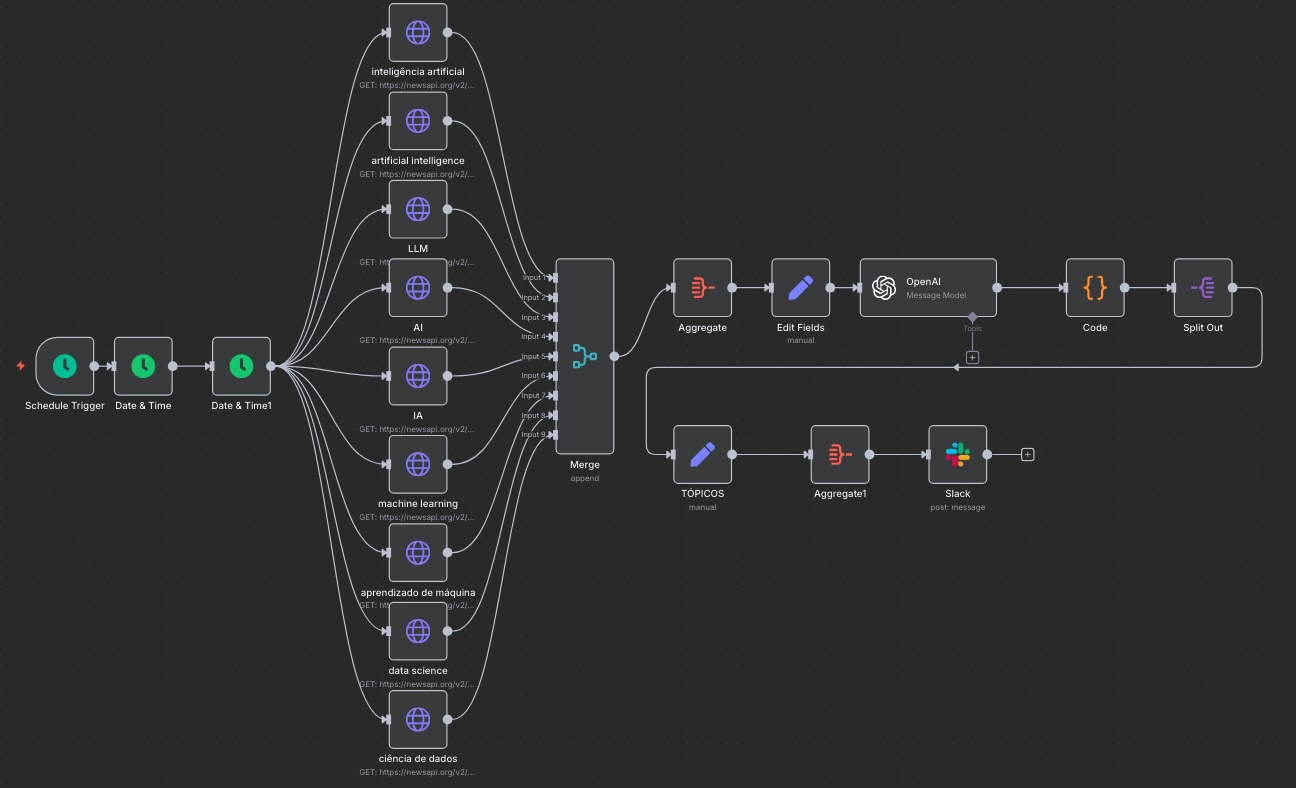
\includegraphics[width=0.8\textwidth]{n8n_workflow.jpg}
    \caption{Diagrama do workflow do n8n para curadoria automatizada de notícias de IA}
    \label{fig:n8n_workflow}
\end{figure}

\section{Principais nós utilizados}

O workflow utiliza diversos nós nativos do n8n, cada um com funcionalidades específicas:

\subsection{Schedule Trigger}
\textbf{Função:} Dispara automaticamente a execução do workflow em horários programados.\\
\textbf{Configuração:} Configurado para executar diariamente às 7h~\cite{n8n_schedule_trigger}.

\subsection{Date \& Time}
\textbf{Função:} Manipula datas e horários, permitindo operações como subtração e formatação.\\
\textbf{Uso no workflow:} Dois nós são utilizados - um para subtrair 1 dia da data atual e outro para formatar no padrão yyyy-MM-dd~\cite{n8n_datetime}.

\subsection{HTTP Request}
\textbf{Função:} Realiza requisições HTTP para APIs externas.\\
\textbf{Uso no workflow:} Nove nós fazem consultas paralelas à NewsAPI com diferentes termos de busca~\cite{n8n_http_request}.

\subsection{Merge}
\textbf{Função:} Combina dados de múltiplas entradas em um único fluxo.\\
\textbf{Configuração:} Configurado para receber 9 entradas (uma de cada consulta à NewsAPI)~\cite{n8n_merge}.

\subsection{Aggregate}
\textbf{Função:} Agrega dados de múltiplos itens em uma única estrutura.\\
\textbf{Uso no workflow:} Dois nós agregam artigos e tópicos formatados respectivamente~\cite{n8n_aggregate}.

\subsection{Edit Fields (Set)}
\textbf{Função:} Modifica, adiciona ou remove campos dos dados.\\
\textbf{Uso no workflow:} Prepara dados para o OpenAI e formata tópicos para o Slack~\cite{n8n_set}.

\subsection{OpenAI}
\textbf{Função:} Integração com modelos de linguagem da OpenAI.\\
\textbf{Configuração:} Utiliza o modelo GPT-4o-mini com prompt personalizado para filtrar e resumir notícias~\cite{n8n_openai}.

\subsection{Code}
\textbf{Função:} Executa código JavaScript personalizado para processamento de dados.\\
\textbf{Uso no workflow:} Processa a resposta JSON do OpenAI, removendo formatação markdown~\cite{n8n_code}.

\subsection{Split Out}
\textbf{Função:} Divide um array em itens individuais para processamento separado.\\
\textbf{Uso no workflow:} Separa o array de notícias em itens individuais~\cite{n8n_split_out}.

\subsection{Slack}
\textbf{Função:} Envia mensagens para canais do Slack.\\
\textbf{Configuração:} Configurado com bot personalizado e emoji para enviar resumo formatado~\cite{n8n_slack}.

\section{Integração do modelo de linguagem}

A integração do modelo de linguagem representa o componente central de inteligência do workflow, sendo responsável por transformar centenas de artigos brutos em um resumo conciso e relevante.

\subsection{Modelo Utilizado}
O workflow utiliza o modelo \textbf{GPT-4o-mini}~\cite{openai_gpt4o_mini} da OpenAI~\cite{openai_api}, acessado através do nó OpenAI do n8n. Esta escolha foi motivada pelo equilíbrio entre capacidade de processamento, custo-benefício e velocidade de resposta, sendo adequado para tarefas de sumarização e filtragem de conteúdo.

\subsection{Configuração do Prompt}
O prompt foi cuidadosamente elaborado para atender às necessidades específicas da empresa:

\begin{itemize}
    \item \textbf{Contexto empresarial:} O modelo é instruído a assumir o papel de um colaborador de uma empresa de tecnologia especialista em IA
    \item \textbf{Critérios de filtragem:} Priorização de notícias relacionadas a desenvolvimento de software, melhoria de processos e aplicações para o agronegócio
    \item \textbf{Filtragem de conteúdo:} Exclusão automática de conteúdo ofensivo, violento ou inadequado
    \item \textbf{Formato de saída:} Estrutura JSON padronizada com campos específicos (número, data, título, resumo, fonte e link)
    \item \textbf{Limitações de tamanho:} Resumos limitados a 450 caracteres para facilitar a leitura
    \item \textbf{Tradução automática:} Todos os conteúdos são traduzidos para português
\end{itemize}

\subsection{Processamento dos Dados}
O modelo recebe como entrada todos os artigos coletados pelas nove consultas à NewsAPI~\cite{newsapi}, totalizando potencialmente centenas de notícias. O processo de inteligência artificial inclui:

\begin{enumerate}
    \item \textbf{Análise de relevância:} Avaliação de cada artigo quanto à sua importância para o contexto empresarial
    \item \textbf{Filtragem temática:} Seleção apenas de conteúdos relacionados a IA, ML e suas aplicações
    \item \textbf{Ranking por importância:} Classificação das notícias por relevância e impacto potencial
    \item \textbf{Sumarização:} Criação de resumos concisos mantendo as informações essenciais
    \item \textbf{Formatação estruturada:} Organização do resultado em formato JSON padronizado
\end{enumerate}

\subsection{Pós-processamento}
Após a resposta do modelo, o nó \textit{Code} processa o JSON retornado, removendo formatação markdown desnecessária e preparando os dados para os passos subsequentes do workflow. Esta etapa garante que a estrutura de dados esteja limpa e pronta para formatação final.

\section{Conclusões e aprendizados obtidos}

O desenvolvimento deste workflow automatizado para curadoria de notícias de IA proporcionou diversos aprendizados técnicos e estratégicos relevantes.

\subsection{Eficiência na Automação}
A implementação demonstrou como ferramentas no-code como o n8n~\cite{n8n_platform} podem rapidamente transformar processos manuais repetitivos em fluxos automatizados sofisticados. O que anteriormente demandava horas diárias de trabalho manual agora é executado automaticamente em poucos minutos, liberando recursos humanos para atividades de maior valor agregado.

\subsection{Potencial dos Modelos de Linguagem}
A integração do GPT-4o-mini revelou-se extremamente eficaz para tarefas de filtragem e sumarização de conteúdo. O modelo demonstrou capacidade notável de compreender contexto empresarial específico, aplicar critérios de relevância complexos e produzir resumos concisos mantendo as informações essenciais. A tradução automática e formatação estruturada adicionaram valor significativo ao processo.

\subsection{Arquitetura Escalável}
A estrutura pipeline implementada mostrou-se robusta e facilmente extensível. A coleta paralela de dados de múltiplas fontes, seguida de agregação e processamento centralizado, permite fácil adição de novas fontes de dados ou modificação de critérios de filtragem sem impactar outras partes do sistema.

\subsection{Integração com Ferramentas Empresariais}
A integração direta com Slack~\cite{slack_platform} demonstrou como workflows automatizados podem se integrar seamlessly ao ambiente de trabalho existente, garantindo que informações relevantes sejam entregues no momento e local adequados para a equipe.

\subsection{Limitações Identificadas}
Durante o desenvolvimento, algumas limitações foram observadas:
\begin{itemize}
    \item Dependência de APIs externas (NewsAPI) pode gerar falhas ou limitações de quota
    \item Qualidade dos resumos depende da qualidade dos artigos originais
    \item Necessidade de ajustes periódicos no prompt conforme mudanças no contexto empresarial
    \item Custos operacionais com APIs de IA devem ser monitorados
\end{itemize}

\subsection{Aplicabilidade Futura}
Os conceitos e técnicas aplicados neste projeto são facilmente transferíveis para outras necessidades empresariais, como monitoramento de concorrentes, análise de tendências de mercado, ou curadoria de conteúdo técnico específico. A combinação de ferramentas no-code com inteligência artificial abre possibilidades significativas para automação inteligente de processos empresariais.

% Referências
\bibliographystyle{abntex2-alf}
\bibliography{references}

\end{document}